%%%%%%%%%%%%%%%%%%%%%%%%%%%%%%%%%%%%%%%%%%%%%%%%%%%%%%%
% A template for Wiley article submissions.
% Developed by Overleaf. 
%
% Please note that whilst this template provides a 
% preview of the typeset manuscript for submission, it 
% will not necessarily be the final publication layout.
%
% Usage notes:
% The "blind" option will make anonymous all author, affiliation, correspondence and funding information.
% Use "num-refs" option for numerical citation and references style.
% Use "alpha-refs" option for author-year citation and references style.

\documentclass[num-refs]{wiley-article}
% \documentclass[blind,alpha-refs]{wiley-article}

% Add additional packages here if required
\usepackage{siunitx}
%\usepackage[colorinlistoftodos]{todonotes}
\usepackage{gensymb}

% Update article type if known
\papertype{Full Paper}
% Include section in journal if known, otherwise delete
% \paperfield{Journal Section}

\title{Molybdenum dichalcogenide cathodes for aluminium-ion batteries}

% List abbreviations here, if any. Please note that it is preferred that abbreviations be defined at the first instance they appear in the text, rather than creating an abbreviations list.
% \abbrevs{ABC, a black cat; DEF, doesn't ever fret; GHI, goes home immediately.}

% Include full author names and degrees, when required by the journal.
% Use the \authfn to add symbols for additional footnotes and present addresses, if any. Usually start with 1 for notes about author contributions; then continuing with 2 etc if any author has a different present address.
\author[1]{Shalini Divya}
\author[2\authfn{1}]{Thomas Nann}

\contrib[\authfn{1}]{Corresponding author.}

% Include full affiliation details for all authors
\affil[1]{Victoria University of Wellington, School of Chemical and Physical Sciences, Wellington, New Zealand}
\affil[2]{The University of Newcastle, School of Mathematical and Physical Sciences, Callaghan, NSW 2308, Australia}

%\corraddress{Author One PhD, Department, Institution, City, State or Province, Postal Code, Country}
\corremail{thomas.nann@newcastle.edu.au}

%\presentadd[\authfn{2}]{Department, Institution, City, State or Province, Postal Code, Country}

\fundinginfo{No funding information available.}

% Include the name of the author that should appear in the running header
\runningauthor{Nann et al.}

\begin{document}

\maketitle

\begin{abstract}
Here goes the abstract. This is a generic template designed for use by multiple journals, which includes several options for customization. Please consult the author guidelines for the journal to which you are submitting in order to confirm that your manuscript will comply with the journal's requirements. Please replace this text with your abstract.

% Please include a maximum of seven keywords
%\keywords{aluminium-ion battery, molybdenum disulfide, molybdenum diselenide, ...}

\end{abstract}

\section{Introduction}

\section{Results and Discussion}

Scheme 1 displays the crystal structure of MoX$_2$ where X = S, Se. The molecule has two vacant sites --- M1 and M2. M1 denotes the spaces in between the X-Mo-X bonds whereas M2, a larger site, is denoted by separation of two layers of MoX$_2$ with an inter-layer distance of 6.3\AA. The layers are held at this distance via van-der-Waals (vdW) forces. The M2 site presents an open network and various interstitial sites, which can easily accommodate the AlCl$_4^{-}$ anion, which are 5.28\AA\ in size as reported by Takahashi {\it et al}. An argument can be made about the kind of ion that participates in the intercalation process during charge. Wang {\it et al.} reported participation of Al$^{3+}$ cations, which not only had to overcome their strong electrostatic effect to get in between the layers, but their participation also reduced the reversibility of the redox process by forming complexes with the sulphide ions that remained in the vacant site during discharge. According to our preliminary tests, we found that the participation of Al$^{3+}$ would rather \lq contract\rq\ the MoX$_2$ layers. Density Functional Theory (DFT) studies carried out by Pathak {\it et al.}, showed that AlCl$_4^-$ anions intercalated within the graphite system with its energetically stable tetrahedral form, which is distorted due to the vdW inter-layer attraction forces between the host graphite layers. Here, we propose the intercalation of AlCl$_4^-$ anions into the M2 sites of MoX$_2$ during charging process. The electrochemical results, cyclic voltammetric scans, Raman spectroscopy and X-ray photoelectron spectroscopy results discussed later strongly support the reversible nature of the intercalation process.

\begin{figure}[t]
\centering
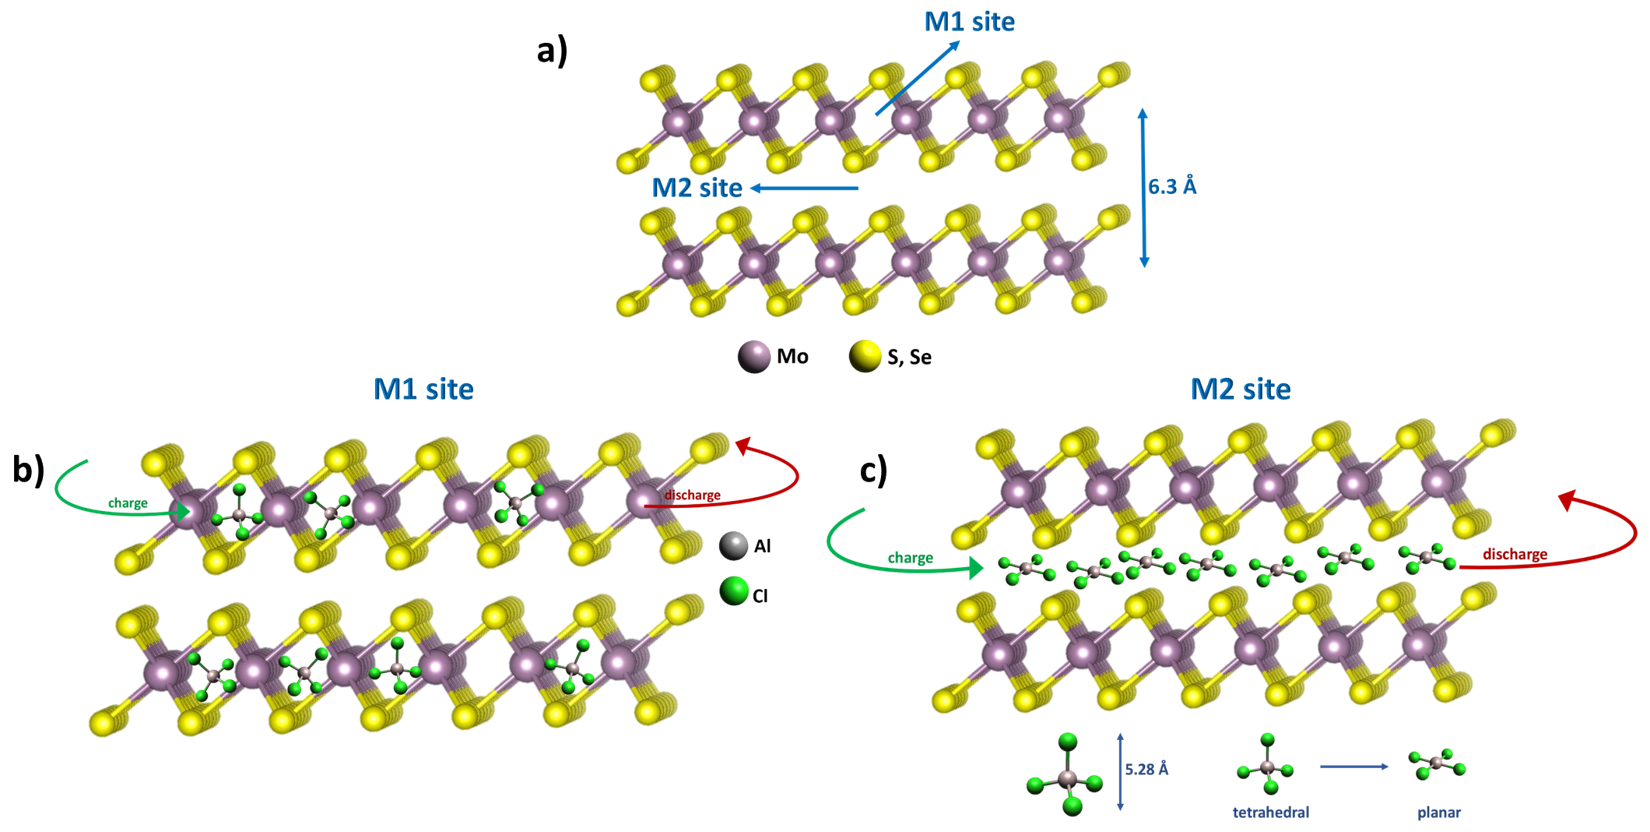
\includegraphics[width=\textwidth]{figures/scheme1}
\caption{Schematic representation of a) an MoX$_2$ crystal structure with possible intercalation sites at M1 and M2 b) intercalation at M1 site and c) intercalation at M2 site.}
\end{figure}

A modified two-electrode polyether ether ketone (PEEK) cell was used to make electrochemical measurements on aluminium-ion batteries (AIBs). Electrode preparations and cell configurations are described in the Methods section. After testing the molybdenum dichalcogenides for AIB cathodes, we found that in general, MoSe$_2$ was superior to MoS$_2$ and MoSSe, with higher and more stable capacities and distinct voltage plateaus. MoSSe was unstable with poor coulombic efficiency of $\sim$50\%. The cathode degraded rapidly after first few cycles and eventually became inactive after a few cycles. It seemed that sulphur substitution weakened the binding energy of Mo-Se allowing the bonds to break easily and thus resulting in rapid cathode degradation and hence, fading capacity. The presence of higher defects in the lattice structure of MoSSe (see XRD and Raman data) compared to MoS$_2$ and MoSe$_2$, contribute to its poor performance as a cathode material in AIBs.

\begin{figure}[h!]
\centering
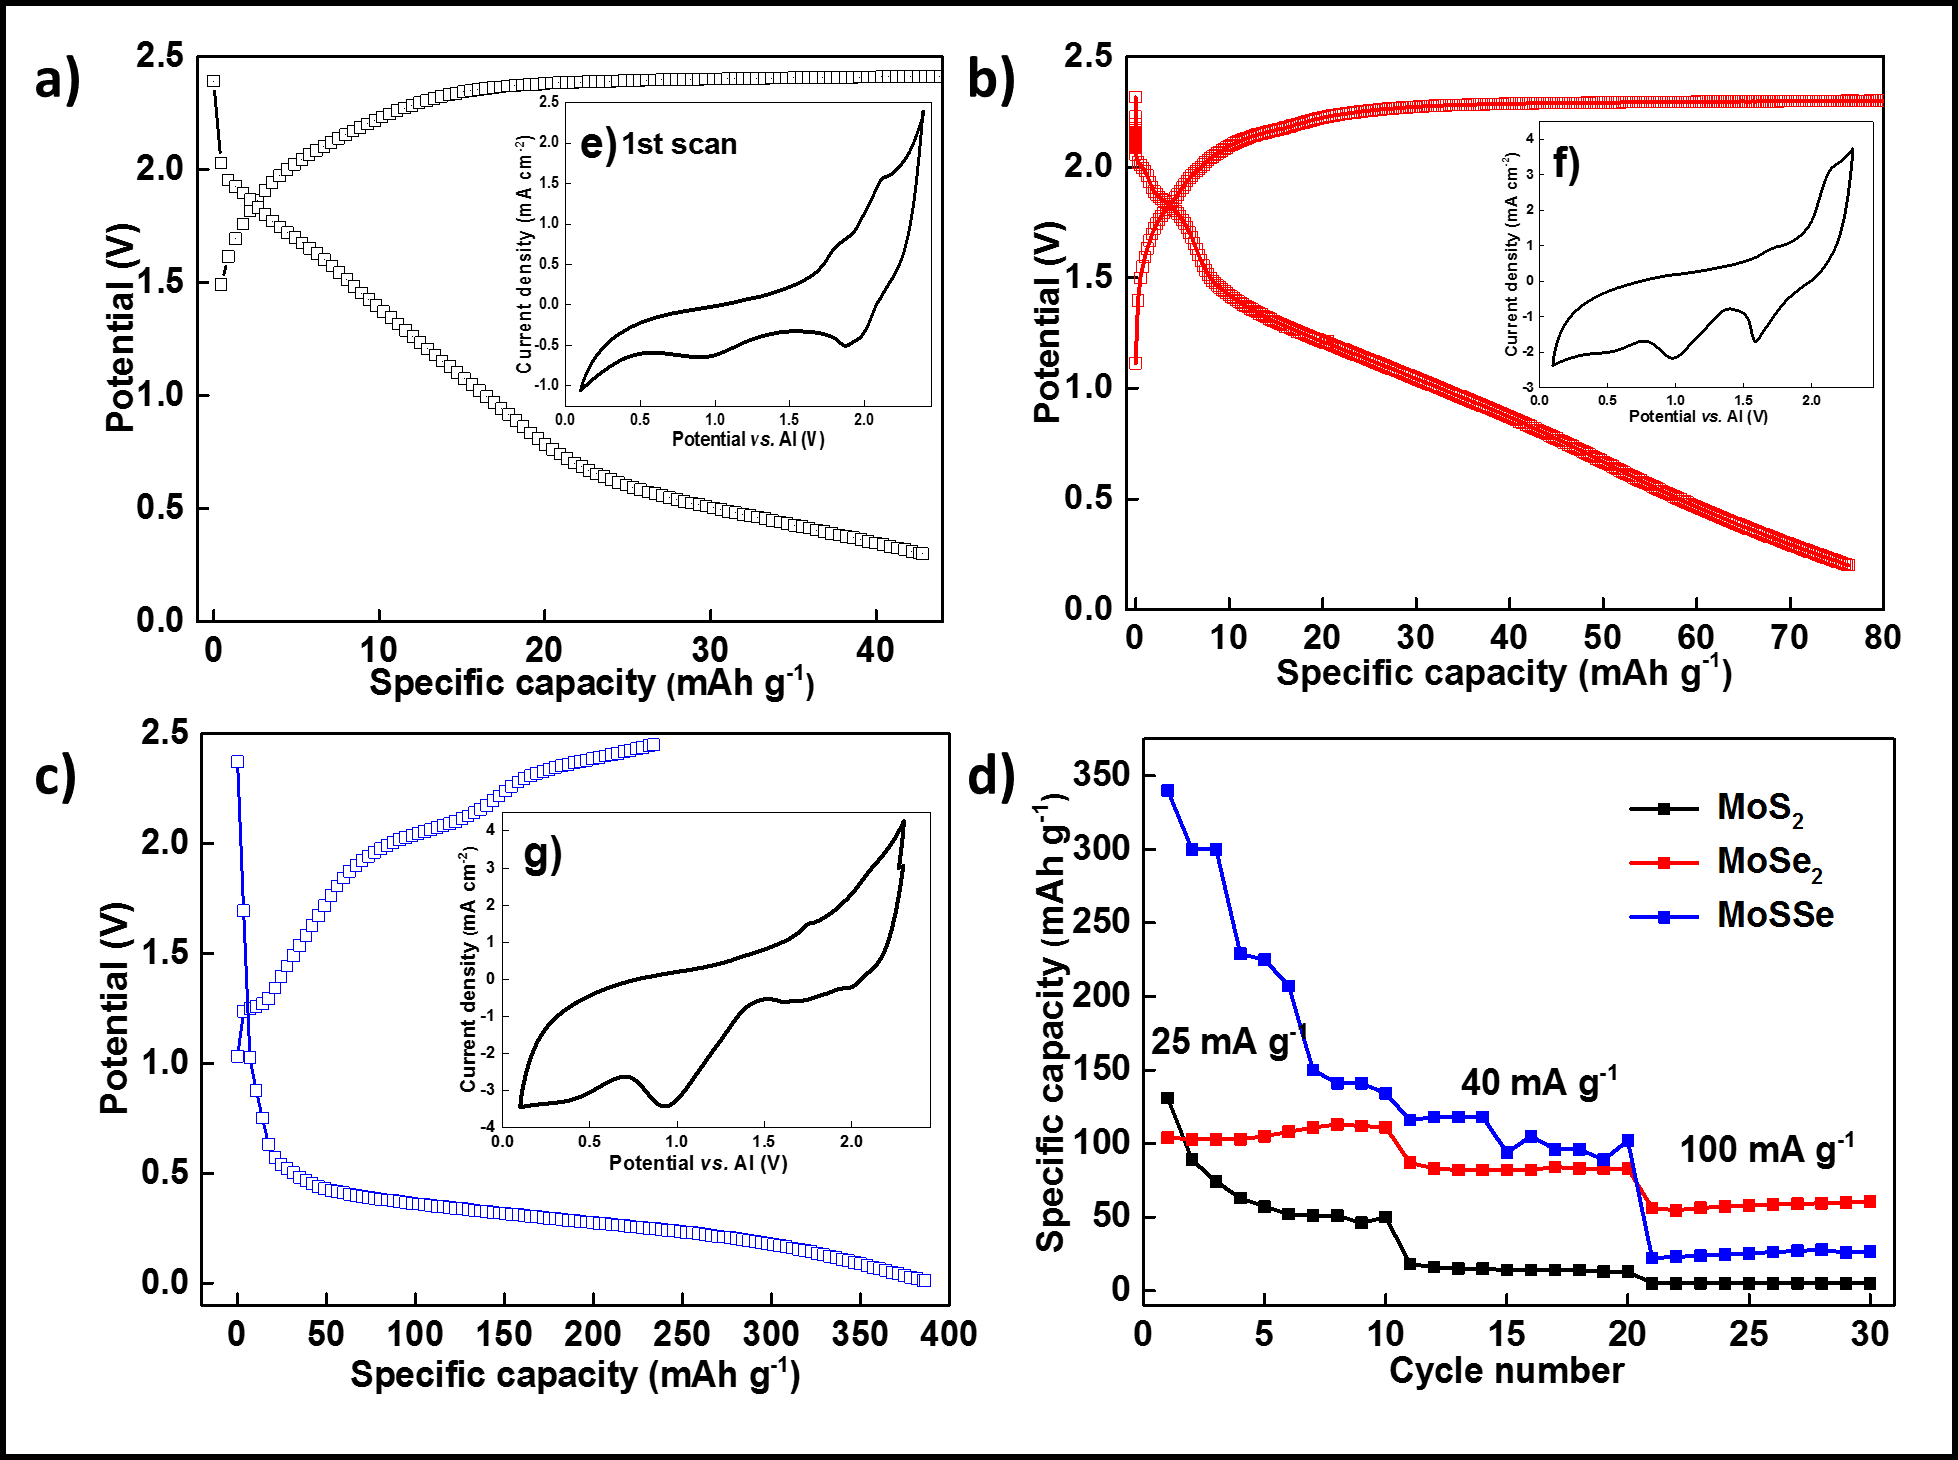
\includegraphics[width=\textwidth]{figures/fig1}
\caption{First charge/discharge curve at 40 mA g$^-^1$ for a) MoS$_2$, b) MoSe$_2$ and c) MoSSe.}
\end{figure}
% Figure 1 here


Figure 1 shows the charge/discharge curves (CDC) for MoS$_2$, MoSe$_2$and MoSSe. The average voltage was observed at 1.8 V for MoS$_2$, 1.7 V for MoSe$_2$ and 0.6 V for MoSSe. For MoS$_2$, capacity after the first discharge was 43 mAh g$^{-1}$, which reduced to 40 mAh g$^{-1}$ and 31 mAh g$^{-1}$ in its second and third cycle respectively. We compared the CDC of the first cycle with their first cyclic voltammetry (CV) scan (Fig 1e) and found a good resemblance between the discharging plateaus (1.9 V and 0.7 V) and reduction peak positions, and in between the charging plateau (2.1 V) and oxidation peak positions. The two-step redox processes have good reversibility, seen in Significant Figure (SF) 1. However, the cell recorded an abnormally high charging capacity in its first cycle. Since intercalation of AlCl$_4^-$ takes places during charging, the irreversible capacity can be attributed to the dissociation of Al$_2$Cl$_7^-$ ions at the electrode surface, or formation of an SEI layer may also render a few side reactions that take place on the electrode-electrolyte interface at such high potentials. CDC for MoSe$_2$ revealed interesting results. With discharge plateaus at 1.9 V and 1.7 V, the first CV scan observed a reduction peak at 1.0 V and 1.65 V. The reduction peak at 1.0 V disappeared after the first scan. This peak can be attributed to an irreversible phase transition that takes place in MoSe$_2$ in its first cycle. During this transition, a semi-conducting 2H phase converts to a more metallic 1T phase.  This transition works in favour of the cathode as it increased the interlayer spacing of MoSe$_2$ (by reducing the vdW forces) and allowing more AlCl$_4^-$ ions to intercalate, thus leading to a higher capacity than MoS$_2$. From the CDC and CV scans, it is apparent that the redox processes are reversible in nature as the discharging plateaus continue to appear at 1.8 V and 2.1 V and charging plateau appears at 2.0 V (Fig S5) after 200 cycle at a current rate of 100 mAg$^{-1}$. A similar phenomenon of high charging capacity during the first cycle was observed and can be similarly attributed to above-mentioned reasons. MoSSe cathode, observed three distinct plateaus during charge at 1.7 V, 2.0 V and 2.3 V in its first cycle with a very low discharge plateau at 0.5 V. The first CV scan revealed a distinct reduction potential at 0.9 V, which disappeared after 1st cycle implying a similar irreversible phase transition. We noticed only one reduction peak at 1.7 V in the consecutive scans and its intensity increased with every cycle. This did not seem to be a part of any redox process as no plateau was observed at that potential in its CDC. An increase in charging capacity during the first three cycles might have been due to... The rate capability test for three electrodes was carried out at various current rates of 25, 40 and 100 mA/g. Lower capacities at higher current rates can be attributed to the decrease in the number of ions transferred in between the electrode and the electrolyte, which decreases the battery capacity. An increase in resistance at higher current rates can also be a reason why the capacity fades.
\begin{figure}[h!]
\centering
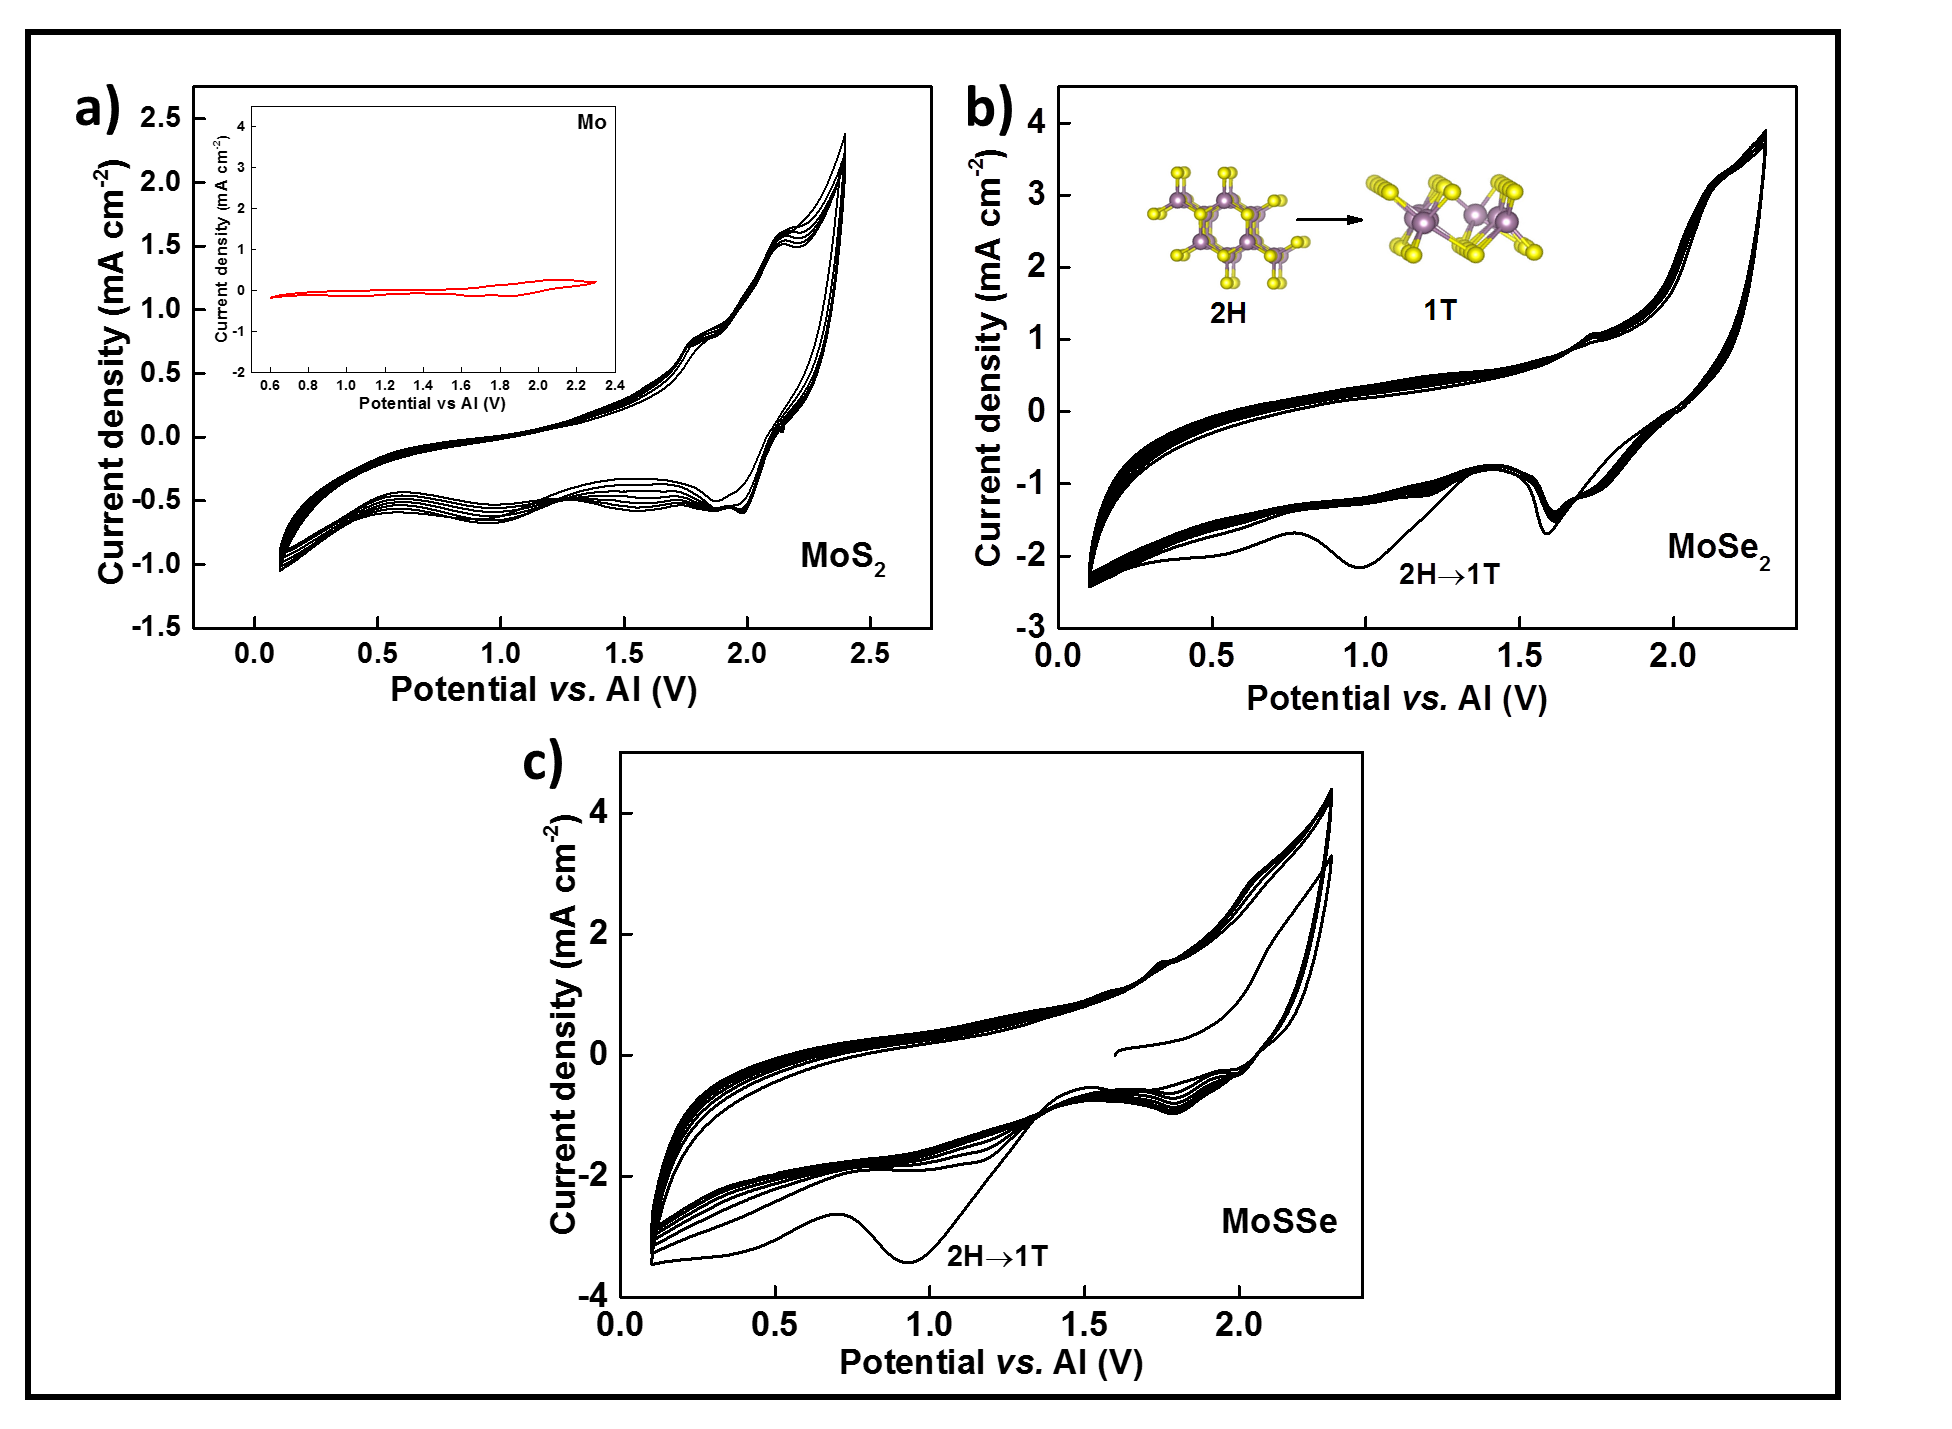
\includegraphics[width=\textwidth]{figures/fig2}
\caption{Cyclic voltammograms of a) MoS$_2$, b) MoSe$_2$ and c) MoSSe at a scan rate of 10 mV s$^-^1$..}
\end{figure}
% Figure 2 here

Both MoS$_2$ and MoSe$_2$ have similar interlayer distance (6.5 \AA) but MoSe$_2$ recorded a higher capacity and a more stable cycle life than MoS$_2$. This behaviour can be attributed to the different charge storage mechanisms the two materials follow. CV curves for MoSe$_2$ (Fig 2b) and MoSSe (Fig 2c) have a higher area than MoS$_2$ (Fig 2a) and a more rectangular shape suggesting an additional electrocapacitive mechanism. Charge storage in MoS$_2$ is primarily based on reversible intercalation of AlCl$_4^-$ ions during charge at 1.9 V (Fig S1). MoSe$_2$ showed an intercalation process and an electric double-layer charge storage at the electrode-electrolyte interface, resulting in a higher capacity and a high area under the CV curve. In addition, the phase transition for MoSe$_2$ and MoSSe (2H$\rightarrow$1T) is prominent in their first cycle at 0.9 V. No such transitions were observed for MoS$_2$. CV scan of MoSSe, which lacked any reversible redox peaks, revealed the capacity is mainly focused on non-Faradaic behaviour.

\begin{figure}[h!]
\centering
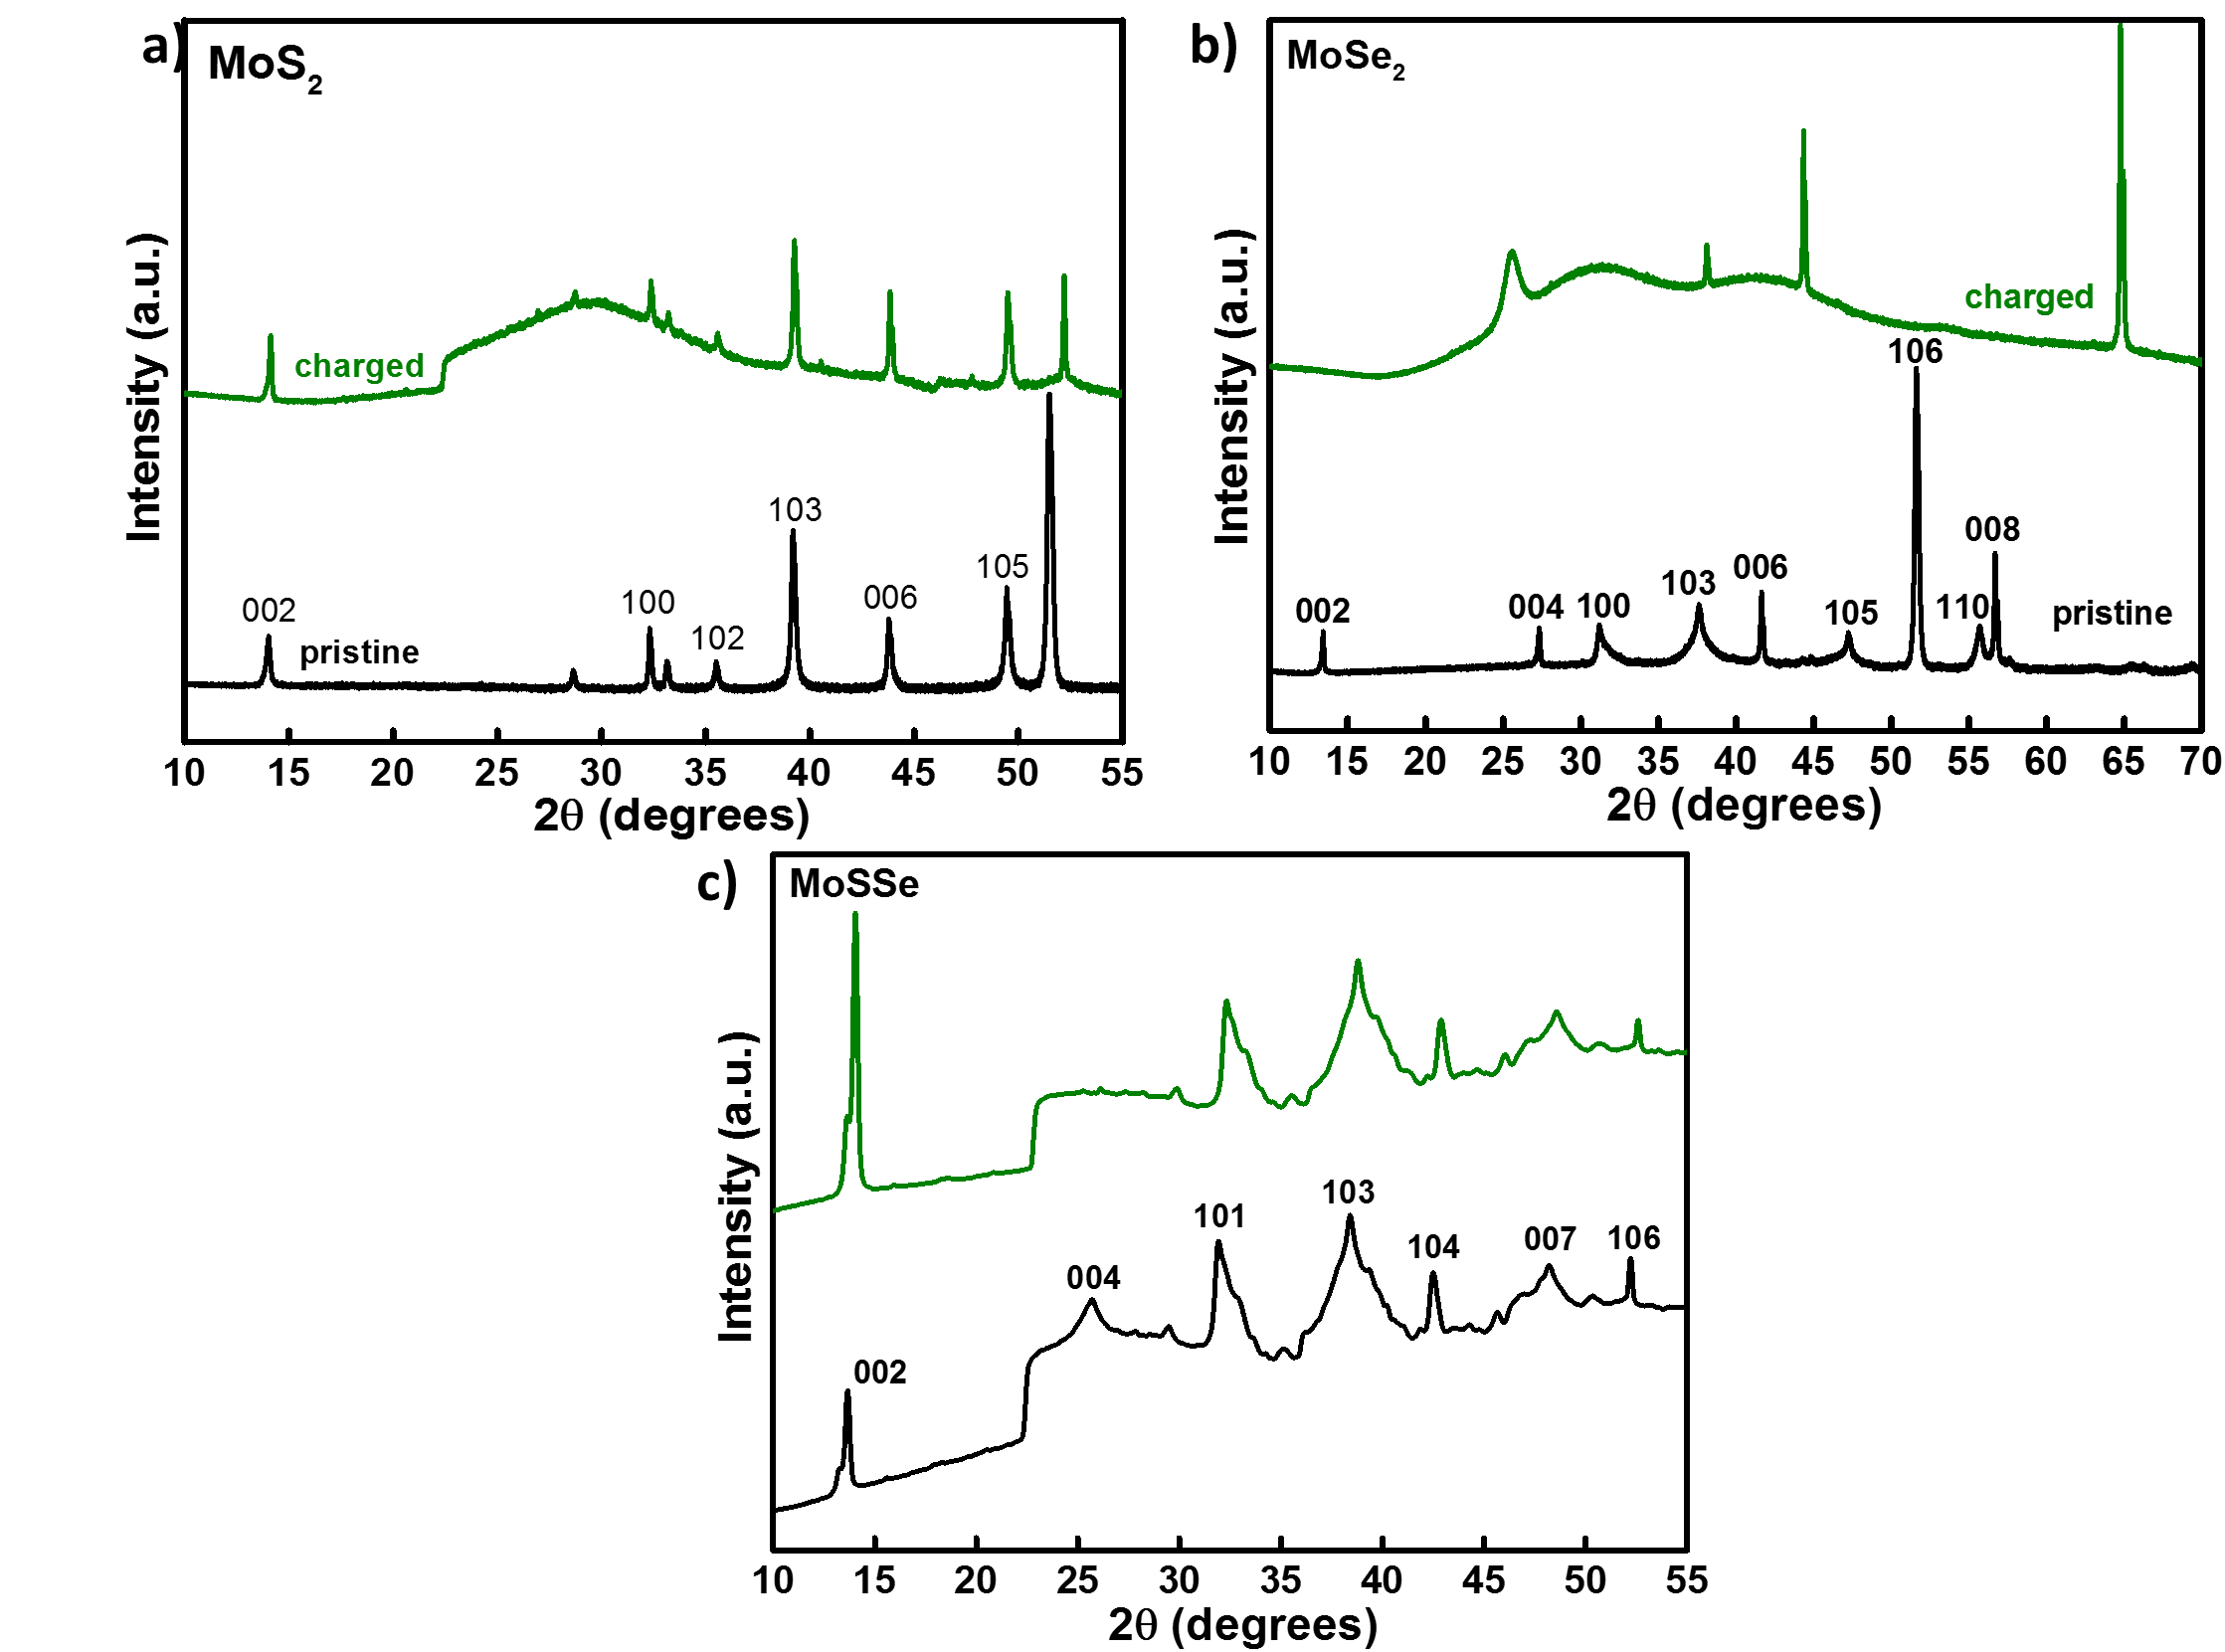
\includegraphics[width=\textwidth]{figures/fig3}
\caption{X-ray diffraction spectra of pristine (black) and charged (green) a) MoS$_2$, b) MoSe$_2$ and c) MoSSe.}
\end{figure}
%Figure 3 here....

Figure 3 displays the X-ray diffraction measurements of MoSe$_2$ and MoSSe electrodes cycled at current rate of 40 mA g$^{-1}$. XRD spectra for MoS$_2$ (Fig S6) compares the pristine (verified by JCPDS No. 17-0744) and charged electrode. The 002 plane (along the c-axis of MoS$_2$) shifted from 14.21\degree\  to 14.02\degree. MoSe$_2$ displayed significantly broadened peaks after charge. The diffraction peak at 2$\theta$ values of 13.4\degree\ (002) disappeared after charging, whereas the peaks at  27.28\degree\ (004), 41.64\degree\ (006) and 51.59\degree\ (106) shifted to 25.58\degree\ , 38.08\degree\  and 44.38\degree\ respectively. The 004 and 006 planes are along the c-axis of the molecule and a decrease in their theta values indicates an increase in the interlayer spacings. This confirms the intercalation of planar AlCl$_4^-$ ions. A new diffraction peak was observed at 44.38\degree, which can be attributed to a new intercalation complex formed after intercalation of AlCl$_4^-$. MoSSe, however, does not have a well-defined crystal structure, which is evident from its diffraction pattern (Fig 3b). The defects might have formed during sulphur substitution in the Mo-Se bond making the Mo-Se bond weaker, which is why the cathode starts to degrade after a few cycles. Interestingly, the 004 plane at 26\degree\ disappears after discharge.

\begin{figure}[h!]
\centering
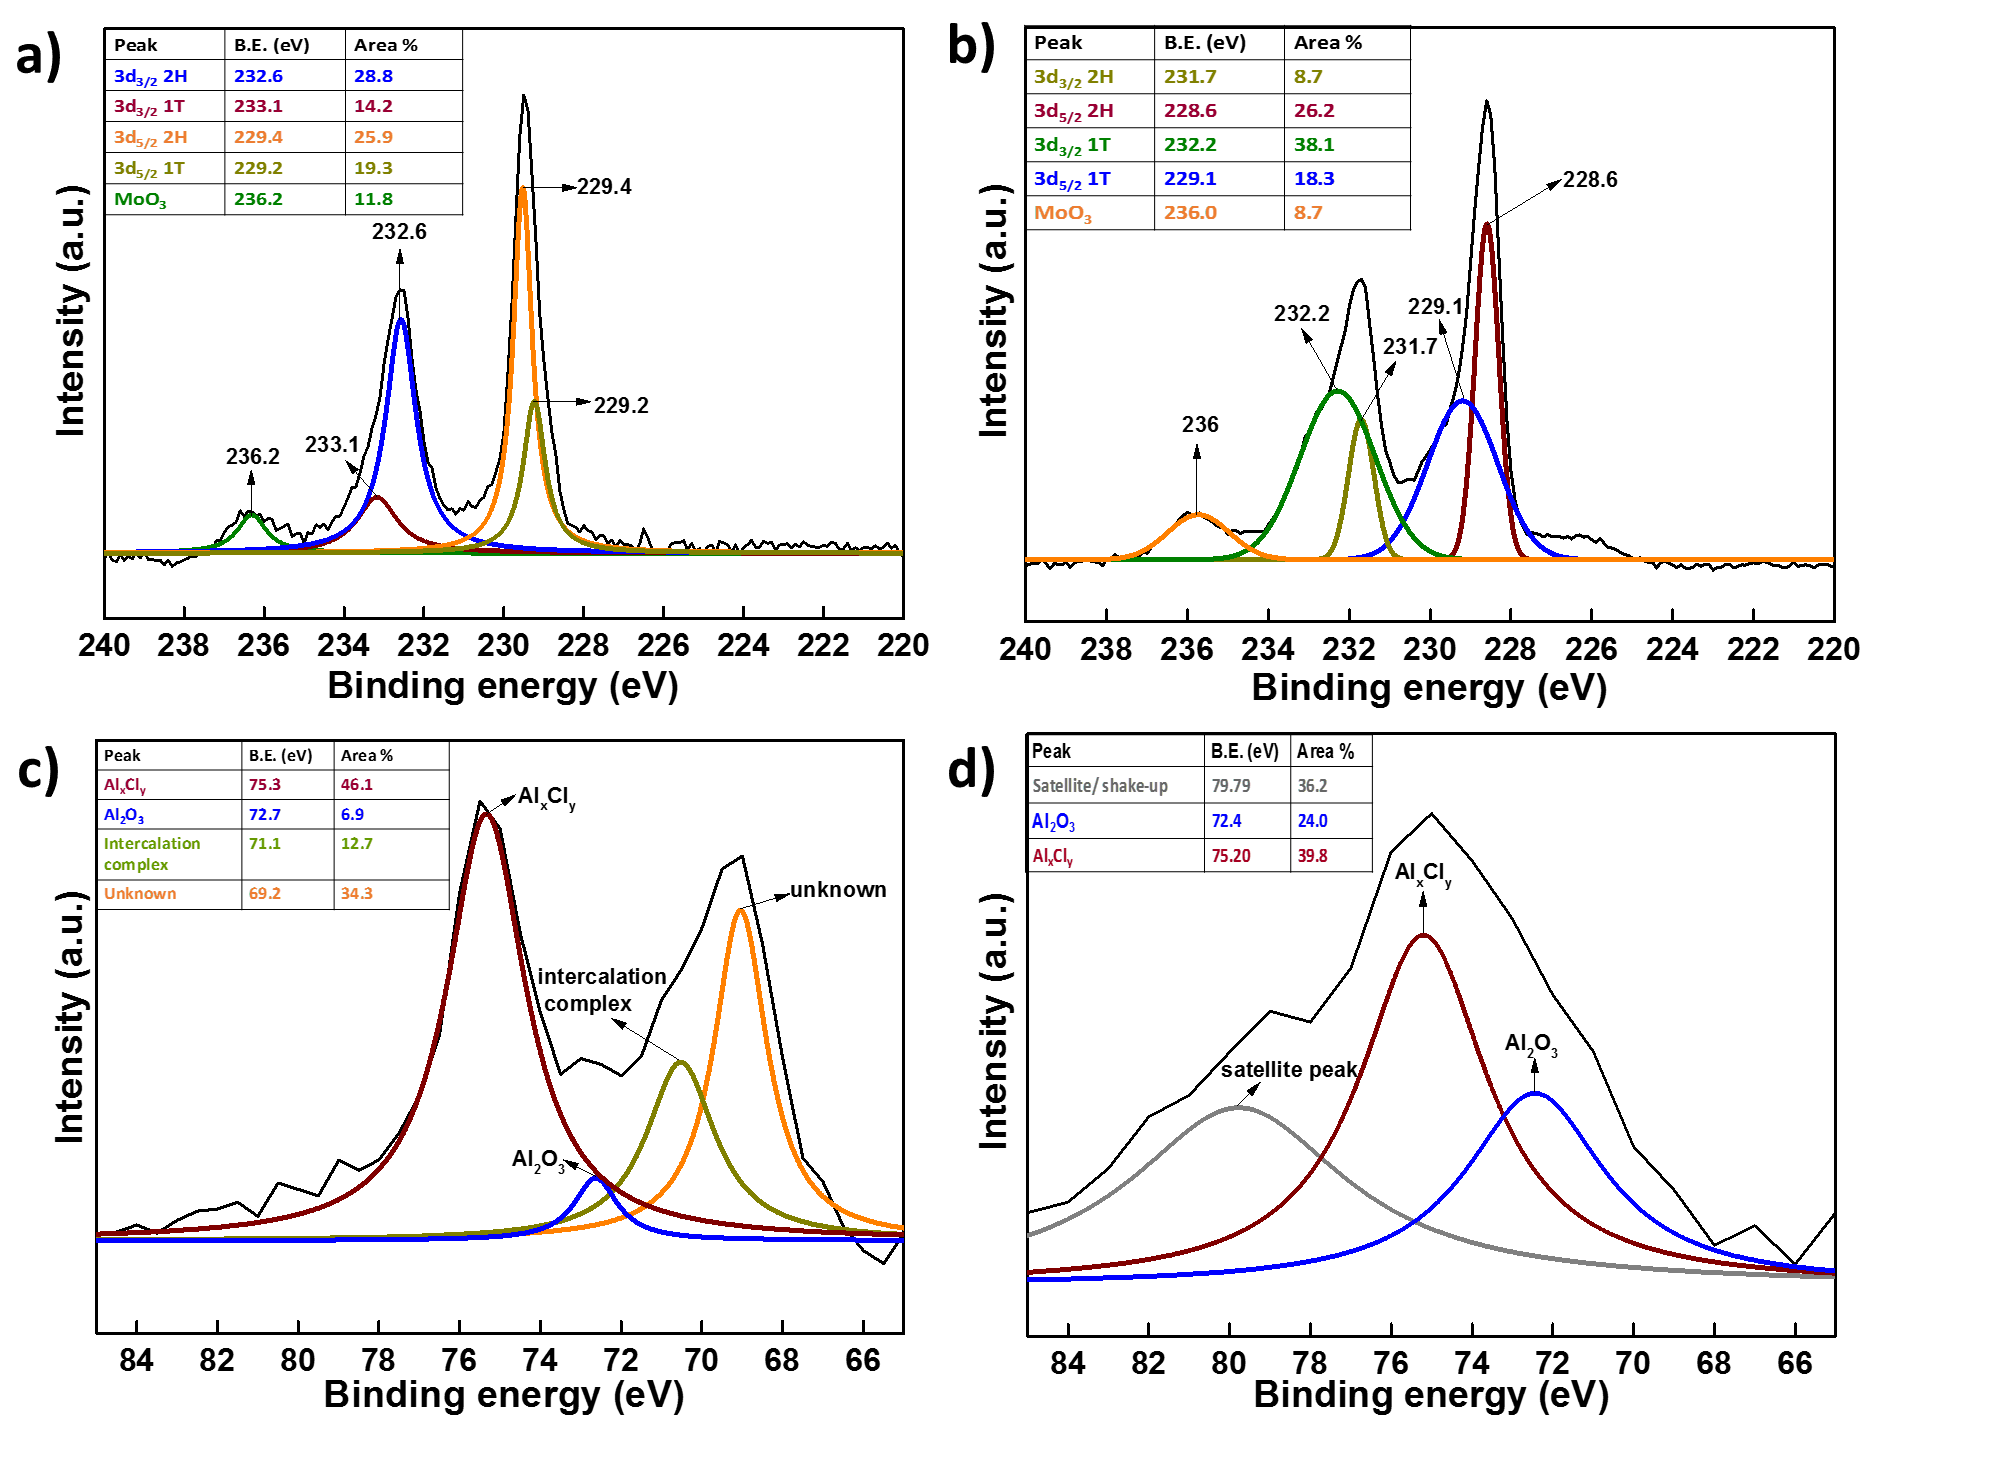
\includegraphics[width=\textwidth]{figures/fig4}
\caption{XPS spectra of Mo 3d orbital in a charged a) MoSe$_2$ and b) MoSSe electrode and Al 2p orbital in a charged c) MoSe$_2$ and d) MoSSe electrode.}
\end{figure}
% Figure 4 here.

To further establish the phase transition effect in MoSe$_2$- X-ray photoelectron spectroscopy (XPS) was used, which is a useful tool in distinguishing different polymorphs (2H and 1T) and oxidation states of transition metal dichalcogenides. Detailed narrow spectrum scan (Figure 4) displays the binding energy of Mo (3d5/2 and 3d3/2), S (2p3/2 and 2p1/2), Se (3d5/2 and 3d3/2) and Al 2p peaks for charged MoSe$_2$ and MoSSe electrodes. The binding energies for Mo 3d in pristine in MoSe$_2$ and MoSSe were observed at 229.4 eV and 232.6 eV (Fig S7a) corresponding to Mo$^{4+}$ 3d5/2 and Mo$^{4+}$ 3d3/2 from the 2H polymorph. Any shift in binding energy or peak splitting in an XPS spectrum can be used to detect phase change or a change in oxidation states of an element. Binding energies of sulphur at 163.5 eV and 162.6 eV corresponding to 2p1/2 and 2p3/2 respectively, did not record any peak shift (Fig S8a and b). For pristine MoSe$_2$ electrodes, the binding energy of Mo 3d observed two peaks at 229.1 eV and 232.2 eV corresponding to 3d5/2 and 3d3/2 and Se 3d included a doublet at 55.4 eV and 54.6 eV corresponding to Se 3d3/2 and 3d5/2 respectively (Fig S9a and b). The peak for Mo 3d3/2 split into two peaks at 233.1 eV and 232.6 eV and Mo 3d 5/2 split into 229.4 eV and 229.2 eV (Fig 4a) after the electrodes were charged. Peak for Se 3d3/2 at 55.4 eV split into 56.0 eV and 55.7 eV (Fig S9b). The peak splitting implies presence of higher oxidation states (Mo$^{4+}$ $\rightarrow$ Mo6+) states and transformation of MoSe$_2$ in 2H phase to a more conducting 1T phase. In the pristine electrode of MoSSe, spectra for Mo 3d (Fig S10) and Se 3d deconvoluted into multiple peaks (Mo$^{4+}$ 3d3/2 into 232.2 eV and 231.7 eV and Mo$^{4+}$ 3d5/2 into 229.1 eV and 228.6 eV) indicating presence of both polymorphs, 2H and 1T, with various oxidation states of Mo (+4 and +6) and Se (+2 and +4). For the MoSSe electrode, peak area increased for Mo 3d peak at 231.7 eV and 228.6 eV corresponding to 3d5/2 and 3d3/2 respectively (Fig . Increase in the 1T polymorph after the first cycle increases the peak areas. In addition, the doublet for Se 3d was replaced by one broad peak, which can be deconvoluted into four peaks at 55.9 eV, 55.2 eV, 54.6 eV and 54.0 eV further confirming the presence of a different polymorph. A new peak at ~236 eV in Mo 3d spectra for MoS$_2$, MoSe$_2$ and MoSSe electrodes (Fig S7b, Fig 4a and 4b) corresponds to Mo6+ species from MoO3 after exposure of the electrode in air. Fig S10 suggests presence of MoO3 in the pristine MoSSe electrode. XPS probing for Al 2p showed presence of Al in all charged electrodes of MoS$_2$ (Fig S12), MoSe$_2$ (Fig 4c) and MoSSe (Fig 4d). The MoSe$_2$ electrode (Fig 4c) displayed binding energies of Al 2p at 77 eV and 76eV corresponding to chlorides (Al$_x$Cl$_y$) and Al2O3 respectively. The oxide formation can be attributed to the passivation of the anode. As AlCl$_4^-$ ions intercalate into MoSe$_2$ layers, a new peak at 69 eV was detected indicating formation of a new complex. MoSSe electrode displayed broad peaks at 74.5 eV and 76 eV (Fig 4d) indicating large amount of Al2O3 and chloroaluminate ions respectively. High atomic ratio of AlxCly implies electrolyte residue. Thus, due to increase in 1T phase in both MoS$_2$ and MoSe$_2$, it becomes easier for the AlCl$_4^-$ ions to intercalate in between its layers. 

\begin{figure}[h!]
\centering
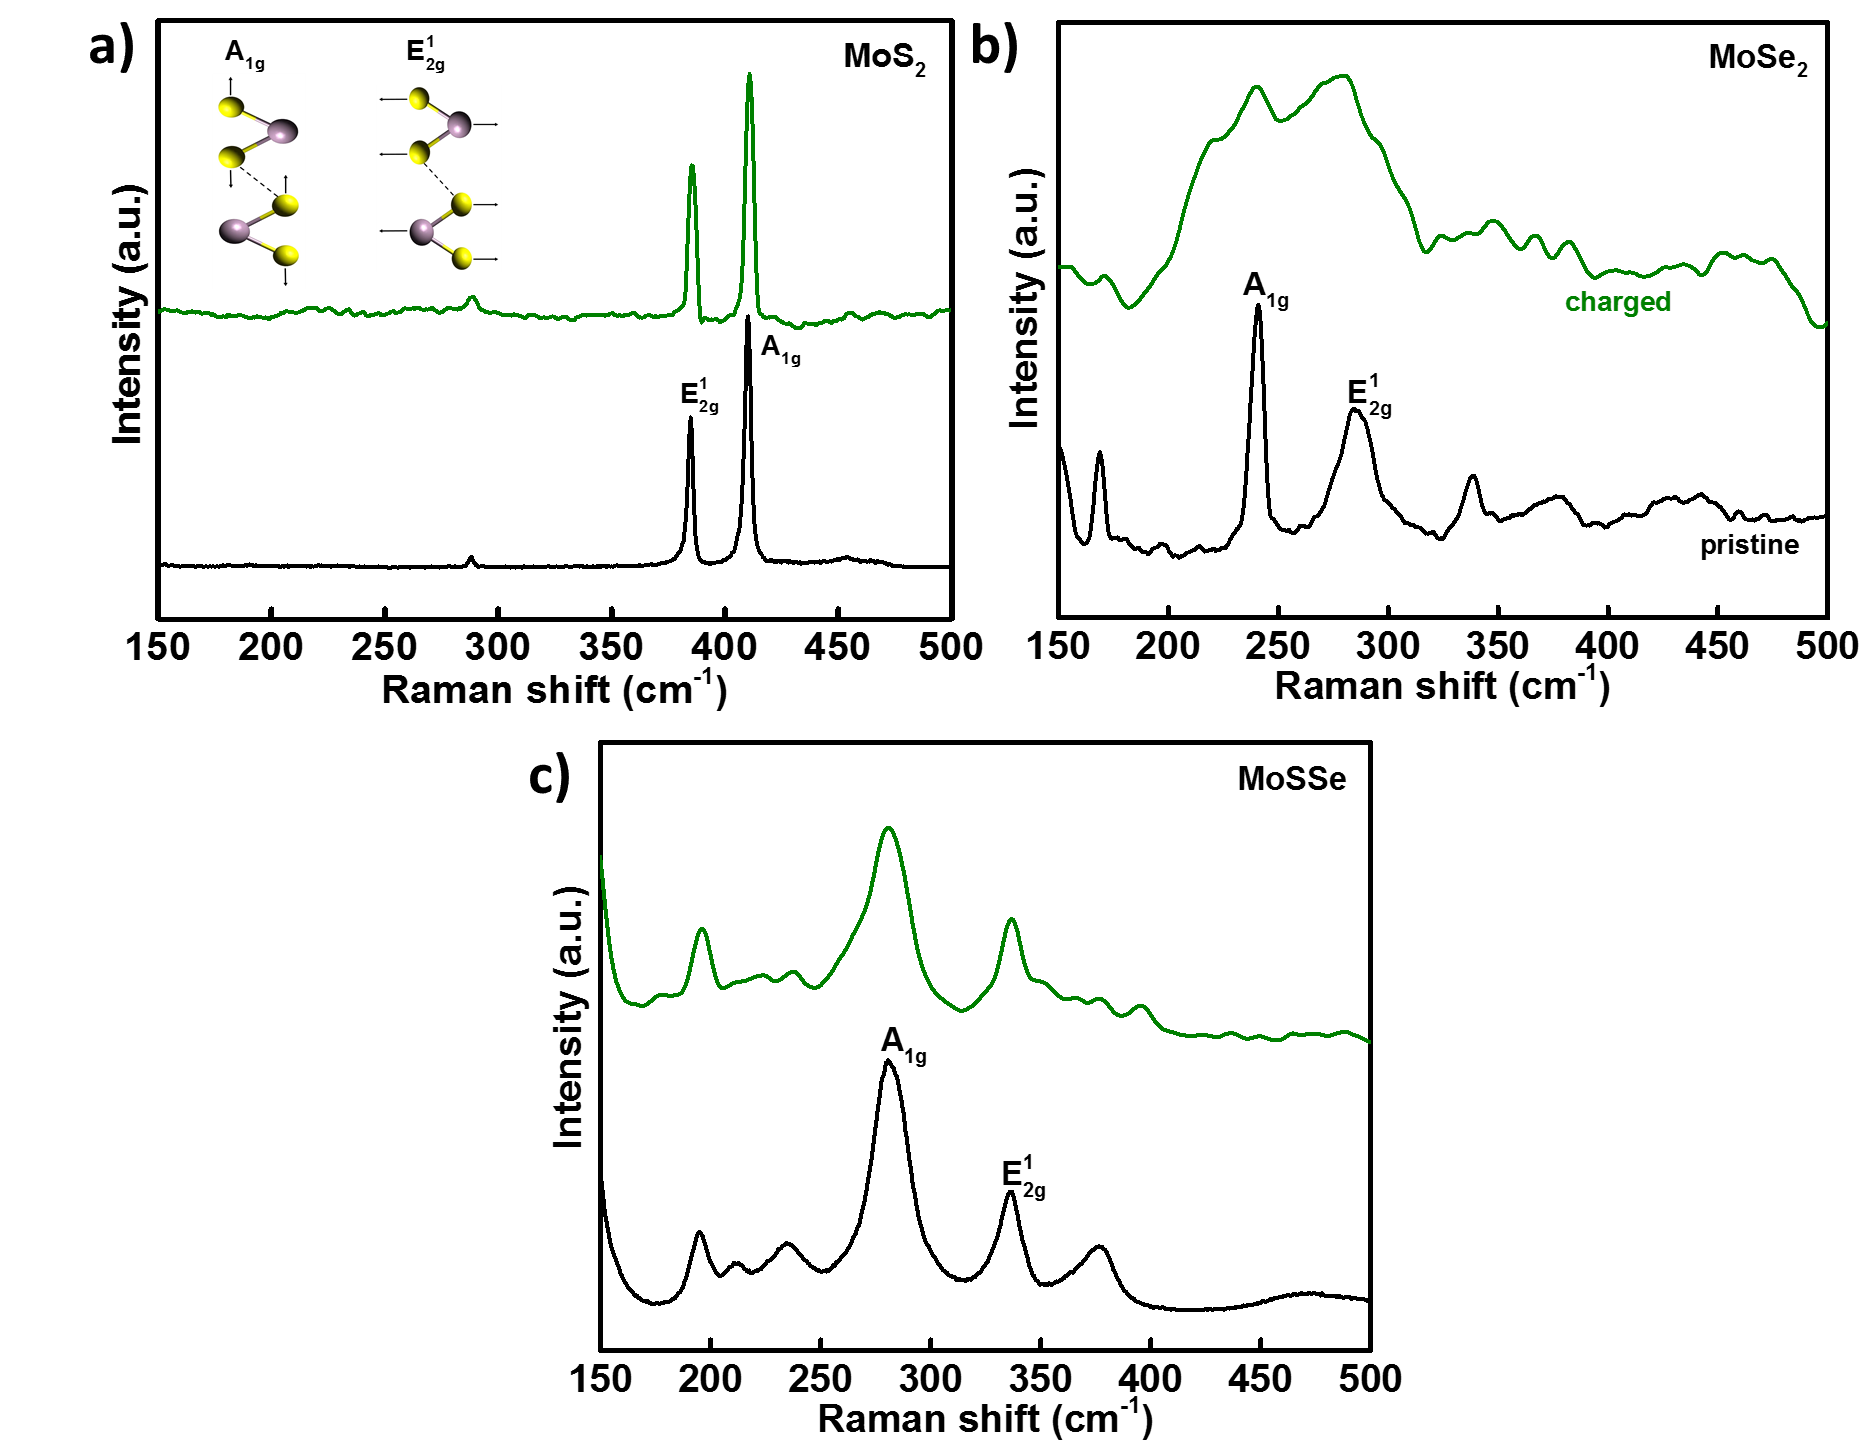
\includegraphics[width=\textwidth]{figures/fig5}
\caption{Raman spectra of pristine (black) and charged (green) a) MoS$_2$, b) MoSe$_2$ and c) MoSSe electrode .}
\end{figure}
% Figure 6 here

We compared the Raman spectra of pristine and charged electrodes of MoSe$_2$ and MoSSe to detect shift in the vibrational modes of the molecule, which would imply presence of polymorphs. Two peaks corresponding to E12g and A1g vibrational modes for MoS$_2$ (Fig S14) are prominent at 384.6 cm$^{-1}$ and 410.2 cm$^{-1}$ respectively. A1g indicates an out-of-plane symmetric displacement of S atoms, whereas E12g suggests an in-layer displacement. A separation between the two modes indicates a multilayer structure, which is observed for all three materials. No significant peak shift was observed for the charged MoS$_2$ electrode implying no phase change. Raman spectra of MoSe$_2$ (Fig 6a) displayed broadening of A1g peak at 240.6 cm$^{-1}$, which shifted to 239.3 cm$^{-1}$ after intercalation of AlCl$_4^-$ ions. E12g peak at 284.5 cm$^{-1}$ shifted to 279.2 cm indicating an increase in lattice defect sites. These shifts and peak broadening correspond to phase transition of MoSe$_2$ from semiconducting 2H phase to more metallic and conducting 1T phase. This confirms with our previous results where we observed phase transition for MoSe$_2$ but not in MoS$_2$. Fig 6b showed the vibrational modes of MoSSe with A1g peak at 281.2 cm$^{-1}$ and E12g at 336.4 cm$^{-1}$. A1g peak in the pristine MoSSe electrode broadened after intercalation of AlCl$_4^-$ ions but the change was not as significant as MoSe$_2$. Raman results help us further establish the fact that MoSe$_2$ underwent significant structural changes allowing better intercalation of AlCl$_4^-$ ions than MoS$_2$. 

\section{Conclusions}

It's all very, very good.

\section{Experimental Section}


\section*{Supporting Information}
Supporting  Information  is  available  from  the  Wiley  Online  Library  or  from the author.

\section*{acknowledgements}
\cite{wang_binder-free_2015}
Acknowledgements should include contributions from anyone who does not meet the criteria for authorship (for example, to recognize contributions from people who provided technical help, collation of data, writing assistance, acquisition of funding, or a department chairperson who provided general support), as well as any funding or other support information. Before I forget it... here is a reference just for Shalini \cite{lahan_al3+_2019, nacimiento_exploring_2018, li_rechargeable_2018, wei_molybdenum_2017, geng_reversible_2015}.

\section*{Conflict of Interest}
The authors declare no conflict of interest.

\section*{Keywords}
Aluminium-ion battery; ...

%Bibliography
\bibliography{zoteroBBT_refs}

\pagebreak

\graphicalabstract{figures/graphical-abstract}{Please check the journal's author guidelines for whether a graphical abstract, key points, new findings, or other items are required for display in the Table of Contents.}


\end{document}


% After this line it is just template stuff - ignore it...
% ----------------------------------------------------------------------

\subsection{Second Level Heading}
If data, scripts or other artefacts used to generate the analyses presented in the article are available via a publicly available data repository, please include a reference to the location of the material within the article.

% Equations should be inserted using standard LaTeX equation and eqnarray environments, not as graphics, and should be set in the main text
This is an equation, numbered
\begin{equation}
\int_0^{+\infty}e^{-x^2}dx=\frac{\sqrt{\pi}}{2}
\end{equation}
And one that is not numbered
\begin{equation*}
e^{i\pi}=-1
\end{equation*}

\subsection{Adding Citations and a References List}

Please use a \verb|.bib| file to store your references. When using Overleaf to prepare your manuscript, you can upload a \verb|.bib| file or import your Mendeley, CiteULike or Zotero library directly as a \verb|.bib| file\footnote{see \url{https://www.overleaf.com/blog/184}}. You can then cite entries from it, like this: \cite{lees2010theoretical}. Just remember to specify a bibliography style, as well as the filename of the \verb|.bib|.

You can find a video tutorial here to learn more about BibTeX: \url{https://www.overleaf.com/help/97-how-to-include-a-bibliography-using-bibtex}.

This template provides two options for the citation and reference list style: 
\begin{description}
\item[Numerical style] Use \verb|\documentclass[...,num-refs]{wiley-article}|
\item[Author-year style] Use \verb|\documentclass[...,alpha-refs]{wiley-article}|
\end{description}

\subsubsection{Third Level Heading}
Supporting information will be included with the published article. For submission any supporting information should be supplied as separate files but referred to in the text.

Appendices will be published after the references. For submission they should be supplied as separate files but referred to in the text.

\paragraph{Fourth Level Heading}
% Here are examples of quotes and epigraphs.
\begin{quote}
The significant problems we have cannot be solved at the same level of thinking with which we created them.\endnote{Albert Einstein said this.}
\end{quote}

\begin{epigraph}{Albert Einstein}
Anyone who has never made a mistake has never tried anything new.
\end{epigraph}

\subparagraph{Fifth level heading}
Measurements should be given in SI or SI-derived units.
Chemical substances should be referred to by the generic name only. Trade names should not be used. Drugs should be referred to by their generic names. If proprietary drugs have been used in the study, refer to these by their generic name, mentioning the proprietary name, and the name and location of the manufacturer, in parentheses.

\begin{table}[bt]
\caption{This is a table. Tables should be self-contained and complement, but not duplicate, information contained in the text. They should be not be provided as images. Legends should be concise but comprehensive – the table, legend and footnotes must be understandable without reference to the text. All abbreviations must be defined in footnotes.}
\begin{threeparttable}
\begin{tabular}{lccrr}
\headrow
\thead{Variables} & \thead{JKL ($\boldsymbol{n=30}$)} & \thead{Control ($\boldsymbol{n=40}$)} & \thead{MN} & \thead{$\boldsymbol t$ (68)}\\
Age at testing & 38 & 58 & 504.48 & 58 ms\\
Age at testing & 38 & 58 & 504.48 & 58 ms\\
Age at testing & 38 & 58 & 504.48 & 58 ms\\
Age at testing & 38 & 58 & 504.48 & 58 ms\\
\hiderowcolors
stop alternating row colors from here onwards\\
Age at testing & 38 & 58 & 504.48 & 58 ms\\
Age at testing & 38 & 58 & 504.48 & 58 ms\\
\hline  % Please only put a hline at the end of the table
\end{tabular}

\begin{tablenotes}
\item JKL, just keep laughing; MN, merry noise.
\end{tablenotes}
\end{threeparttable}
\end{table}

\section*{acknowledgements}
Acknowledgements should include contributions from anyone who does not meet the criteria for authorship (for example, to recognize contributions from people who provided technical help, collation of data, writing assistance, acquisition of funding, or a department chairperson who provided general support), as well as any funding or other support information.

\section*{conflict of interest}
You may be asked to provide a conflict of interest statement during the submission process. Please check the journal's author guidelines for details on what to include in this section. Please ensure you liaise with all co-authors to confirm agreement with the final statement.

\printendnotes

% Submissions are not required to reflect the precise reference formatting of the journal (use of italics, bold etc.), however it is important that all key elements of each reference are included.
\bibliography{sample}

\begin{biography}[example-image-1x1]{A.~One}
Please check with the journal's author guidelines whether author biographies are required. They are usually only included for review-type articles, and typically require photos and brief biographies (up to 75 words) for each author.
\bigskip
\bigskip
\end{biography}

\graphicalabstract{figures/graphical-abstract}{Please check the journal's author guildines for whether a graphical abstract, key points, new findings, or other items are required for display in the Table of Contents.}

%\end{document}
